\documentclass[12pt]{article}
\usepackage[top=1in, bottom=1in, left=.75in, right=.75in]{geometry}
\usepackage{amsmath}
\usepackage{fancyhdr}
\usepackage{graphicx}
\usepackage{txfonts}
\usepackage{multicol,coordsys}
\usepackage[scaled=0.86]{helvet}
\renewcommand{\emph}[1]{\textsf{\textbf{#1}}}
\usepackage{anyfontsize}
\usepackage[shortlabels]{enumitem}
% \usepackage{times}
% \usepackage[lf]{MinionPro}
\usepackage{tikz,pgfplots,mathrsfs}
%\def\degC{{}^\circ{\rm C}}
\def\ra{\rightarrow}
\usetikzlibrary{calc, backgrounds,trees,positioning,arrows,fit,shapes}
\usepackage{pgfplots}
\pgfplotsset{width=9cm,compat=1.9}
\tikzset{
  jumpdot/.style={mark=*,solid},
  excl/.append style={jumpdot,fill=white},
  incl/.append style={jumpdot,fill=blue},
}
%\pgfplotsset{compat = newest}
\newcommand{\blank}[1]{\rule{#1}{0.75pt}}

%\pgfplotsset{my style/.append style={axis x line=middle, axis y line=
%middle, xlabel={$x$}, ylabel={$y$},axis equal}}

%yticklabels={,,} , xticklabels={,,}

% \setmainfont{Times}
% \def\sansfont{Lucida Grande Bold}
\parindent 0pt
\parskip 4pt
\pagestyle{fancy}
\fancyfoot[C]{\emph{\thepage}}
%% version indicator
\fancyfoot[R]{\emph{v2}}
\fancyhead[L]{\ifnum \value{page} > 1\relax\emph{Math 252: Final Exam}\fi}
\fancyhead[R]{\ifnum \value{page} > 1\relax\emph{Fall 2025}\fi}
\headheight 15pt
\renewcommand{\headrulewidth}{0pt}
\renewcommand{\footrulewidth}{0pt}
\let\ds\displaystyle
\def\continued{{\emph {Continued....}}}
\def\continuing{{\emph {Problem \arabic{probcount} continued....}}\par\vskip 4pt}


\newcounter{probcount}
\newcounter{subprobcount}
\newcommand{\thesubproblem}{\emph{\alph{subprobcount}.}}
\def\problem#1{\setcounter{subprobcount}{0}%
\addtocounter{probcount}{1}{\emph{\arabic{probcount}.\hskip 1em(#1)}}\par}
\def\subproblem#1{\par\hangindent=1em\hangafter=0{%
\addtocounter{subprobcount}{1}\thesubproblem\emph{#1}\hskip 1em}}
\def\probskip{\vskip 10pt}
\def\medprobskip{\vskip 2in}
\def\subprobskip{\vskip 45pt}
\def\bigprobskip{\vskip 4in}

\begin{document}
{\emph{\fontsize{26}{28}\selectfont Math F252\hfill
{\fontsize{32}{36}\selectfont Final Exam}
\hfill Fall 2025}}
\vskip 2cm
\strut\vtop{\halign{\emph#\hskip 0.5em\hfil&#\hbox to 2in{\hrulefill}\cr
\emph{\fontsize{18}{22}\selectfont Name:}&\cr
\noalign{\vskip 10pt}}}
%%\emph{\fontsize{18}{22}\selectfont Student Id:}&\cr
%%\noalign{\vskip 10pt}
%%\emph{\fontsize{18}{22}\selectfont Calculator Model:}&\cr
%}}
%\hfill
%\vtop{\halign{\emph{\fontsize{18}{22}\selectfont #}\hfil& \emph{\fontsize{18}{22}\selectfont\hskip 0.5ex $\square$ #}\hfil\cr
%Section: & 001 (Jill Faudree)\cr
%\noalign{\vskip 4pt}
%         & 002 (James Gossell)\cr
%\noalign{\vskip 4pt}
%         & 005 (James Gossell)\cr}}

\vfill
{\fontsize{18}{22}\selectfont\emph{Rules:}}

You have {120 minutes} to complete this midterm.  

Partial credit will be awarded, but you must show your work.

Calculators are not allowed. 

One hand-written sheet of notes is allowed.

%Place a box around your  \fbox{FINAL ANSWER} to each question where appropriate.

%If you need extra space, you can use the back sides of the pages.
%Please make it obvious  when you have done so.

Turn off anything that might go beep during the exam.

Good luck!
\vfill
\def\emptybox{\hbox to 2em{\vrule height 16pt depth 8pt width 0pt\hfil}}
\def\tline{\noalign{\hrule}}
\centerline{\vbox{\offinterlineskip
{
\bf\sf\fontsize{18pt}{22pt}\selectfont
\hrule
\halign{
\vrule#&\strut\quad\hfil#\hfil\quad&\vrule#&\quad\hfil#\hfil\quad
&\vrule#&\quad\hfil#\hfil\quad&\vrule#\cr
height 3pt&\omit&&\omit&&\omit&\cr
&Problem&&Possible&&Score&\cr\tline
height 3pt&\omit&&\omit&&\omit&\cr
&1&&15&&\emptybox&\cr\tline
&2&&6&&\emptybox&\cr\tline
&3&&6&&\emptybox&\cr\tline
&4&&10&&\emptybox&\cr\tline
&5&&20&&\emptybox&\cr\tline
&6&&6&&\emptybox&\cr\tline
&7&&10&&\emptybox&\cr\tline
&8&&10&&\emptybox&\cr\tline
&9&&6&&\emptybox&\cr\tline
&10&&5&&\emptybox&\cr\tline
&11&&6&&\emptybox&\cr\tline
&Extra Credit&&5&&\emptybox&\cr\tline
&Total&&100&&\emptybox&\cr
}\hrule}}}

\newpage
\begin{enumerate}
%% Integration:  IBP ; trig sub ; partial fractions ; 

\item (5 pts each) Evaluate the indefinite integrals. 
	\begin{enumerate}
	\item $\displaystyle \int \dfrac{1}{x^2\sqrt{x^2-4}} dx $
	\vfill

	\item $\displaystyle \int \frac{1}{x^2-9} dx$
	\vfill
\newpage
	\item $\displaystyle \int (4x-xe^x ) dx$
	\vfill
	\end{enumerate}
\item (6 pts) The shaft of a bird feather has density function \fbox{$\rho = \tfrac{2}{5}\arctan x $} grams per meter on the interval from $x=0$ m to $x=1$ m. Find the \emph{mass} of the shaft. \emph{Include units with your answer.}
\vfill
\newpage
\item (6 pts) The region $R$ is bounded by $ y = \sin^2 (x) \cos^3 (x) $ and the x-axis between $x = 0$ and $ x = \pi/2$.  Find the \textbf{area} of the region $R.$

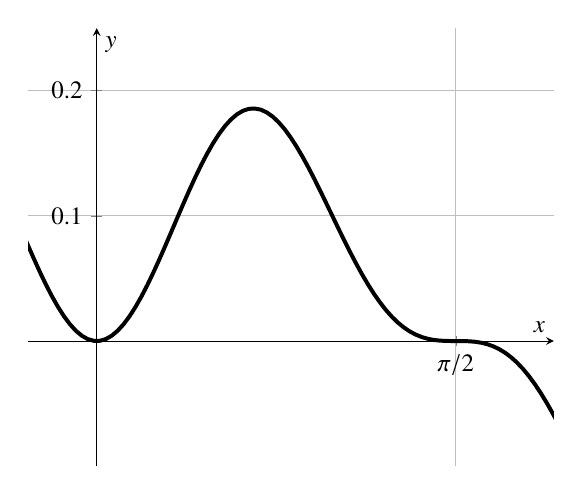
\begin{tikzpicture}[scale = .9]
\begin{axis}[
    axis lines = center,
    xlabel = {$x$},
    ylabel = {$y$},
    xmin = -0.3,
    xmax = 2,
    ymin = -0.1,
    ymax = 0.25,
    samples = 300,
    xtick={-pi/2, 0, pi/2, pi}, % Set tick positions
    ytick={0.1, 0.2}, % Set tick positions
    xticklabels={$-\pi/2$, $0$,  $\pi/2$, $\pi$}, % Label ticks
    xticklabel style={anchor=north}, % Rotate tick labels for better readability
    grid = major]
% Plot the curve
\addplot[<->,ultra thick, black, domain= -3.9:3.9] {(sin(deg(x))^2)*cos(deg(x))*cos(deg(x))*cos(deg(x))};
\end{axis}
\end{tikzpicture}
\vfill



%% Mass (arctan IBP)
\newpage

%% Washers, discs

\item (10 pts) The region $R$ is bounded by $y= e^x$, $y=3$, and the y-axis.
\begin{enumerate}
\item Sketch the region $R.$ Label the curves and all points of intersection of the curves.
\vfill
\item Using either the disks/washers or cylindrical shells method, \emph{set up an integral} to compute the volume generated when $R$ is rotated around the \textbf{$x$-axis}. \emph{State which method you are using.} You do not need to evaluate the integral.
\vfill
\item Using either the disks/washers or cylindrical shells method, \emph{set up an integral} to compute find the volume generated when $A$ is rotated around the \textbf{$y$-axis.} \emph{State which method you are using.} You do not need to evaluate the integral.
\vfill
\end{enumerate}


\newpage

% Series
\item (5 pts each) Determine whether each series below converges or diverges. Name the test you use and justify your conclusion. (This means show your work!)
	\begin{enumerate}
	\item $\displaystyle\sum_{n=1}^{\infty} \cos\left(\frac{1}{5n^2+1}\right)$ \hfill Test: \underline{\hspace{2in}}  \hfill Converge or Diverge\\

	\vfill
	\item $\displaystyle\sum_{n=1}^{\infty} \frac{2+3n}{3+4n^{3/2}}$\hfill Test: \underline{\hspace{2in}}  \hfill Converge or Diverge\\
	
	\vfill
\newpage
	
	\item $\displaystyle\sum_{n=1}^{\infty} \frac{2^n}{n^3}$ \hfill Test: \underline{\hspace{2in}}  \hfill Converge or Diverge\\

	\vfill
	
	\item $\displaystyle\sum_{n=1}^{\infty} \frac{(-1)^n}{\sqrt{3n+2}}$ \hfill Test: \underline{\hspace{2in}}  \hfill Converge or Diverge\\
	\vfill
	\end{enumerate}
\newpage
\item (6 pts) Use the Integral Test to determine whether the series $\displaystyle\sum_{n=2}^{\infty} \frac{1}{n \sqrt{\ln(n)}}$ converges or diverges.
\vfill
\newpage
\item (5 pts each) For each power series below, determine the interval of convergence.
	\begin{enumerate}
	\item $\displaystyle\sum_{n=1}^{\infty} \frac{(x-3)^n}{n5^n}$
	\vfill
	\item $\displaystyle\sum_{n=1}^{\infty} \frac{n!(x+4)^n}{7^{2n}}$
	\vfill
	\end{enumerate}
\newpage
\item (10 pts) Recall that the Maclaurin series \:\:\: $\displaystyle \cos(x) = \sum_{n=0}^\infty \frac{(-1)^n x^{2n}}{(2n)!}.$
	\begin{enumerate}
	\item Write $p_4(x),$ the 4th-degree Maclaurin \emph{polynomial} for $\cos(x).$
	\vfill
	\item Find the Maclaurin series for $f(x)=x \cos(2x).$ Simplify your answer.
	\vfill
	\item Find the Maclaurin series for $G(x) = \int_0^x \cos( \sqrt{t}) \: dt.$
	\vfill
	\vfill
	\end{enumerate}
\vfill
\newpage
\item (6 pts) Consider the curve $x(t) = t^2-3t+1$, $y(t) = e^t.$
\begin{enumerate}[label=(\alph*)]
\item Determine the slope of the curve at the point $(1,1)$.
\vfill
\item Determine the points where the tangent line is horizontal or vertical, or state that none exist.
\vfill
\end{enumerate}
\newpage
\item (5 pts) Make a careful sketch of the polar curve $r = 1 + 2\sin(\theta)$. Label at least 4 points.\\

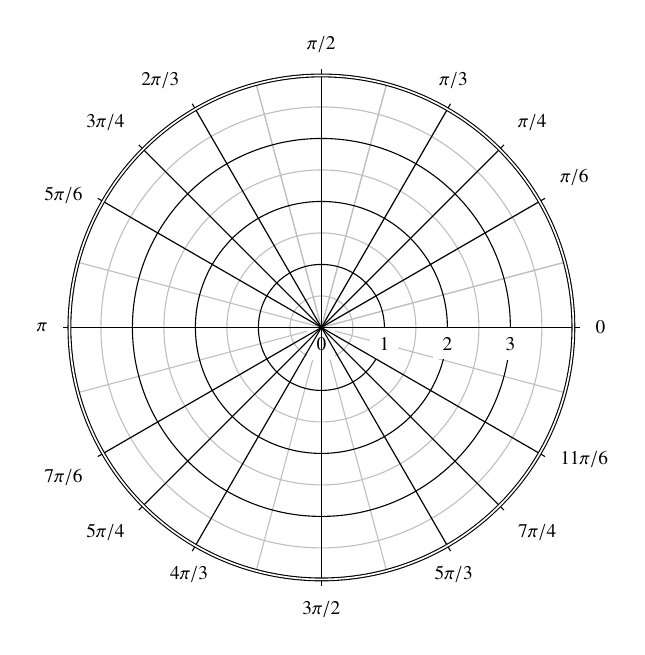
\begin{tikzpicture}[>=latex, scale=.8]
% Draw the lines at multiples of pi/12
\foreach \ang in {0,...,31} {
  \draw [lightgray] (0,0) -- (\ang * 180 / 12:4);
}
% Concentric circles and radius labels
\foreach \s in {0, 1, 2, 3} {
  \draw [lightgray] (0,0) circle (\s + 0.5);
  \draw (0,0) circle (\s);
  \node [fill=white] at (\s, 0) [below] {\scriptsize $\s$};
}
% Add the labels at multiples of pi/4
\foreach \ang/\lab/\dir in {
  0/0/right,
  1/{\pi/4}/{above right},
  2/{\pi/2}/above,
  3/{3\pi/4}/{above left},
  4/{\pi}/left,
  5/{5\pi/4}/{below left},
  7/{7\pi/4}/{below right},
  6/{3\pi/2}/below} {
  \draw (0,0) -- (\ang * 180 / 4:4.1);
  \node [fill=white] at (\ang * 180 / 4:4.2) [\dir] {\scriptsize $\lab$};
}
% Add the labels at multiples of pi/6
\foreach \ang/\lab/\dir in {
  1/{\pi/6}/{above right},
  2/{\pi/3}/above,
  4/{2\pi/3}/{above left},
  5/{5\pi/6}/{left},
  7/{7\pi/6}/{below left},
  8/{4\pi/3}/below,
  10/{5\pi/3}/below,
  11/{11\pi/6}/right} {
  \draw (0,0) -- (\ang * 180 / 6:4.1);
  \node [fill=white] at (\ang * 180 / 6:4.2) [\dir] {\scriptsize $\lab$};
}
% The double-lined circle around the whole diagram
\draw [style=double] (0,0) circle (4);
\end{tikzpicture}
\vfill
\item (6 pts) Compute the area enclosed by the polar curve $r=3 \sin(4 \theta).$ The graph of the curve is shown below.

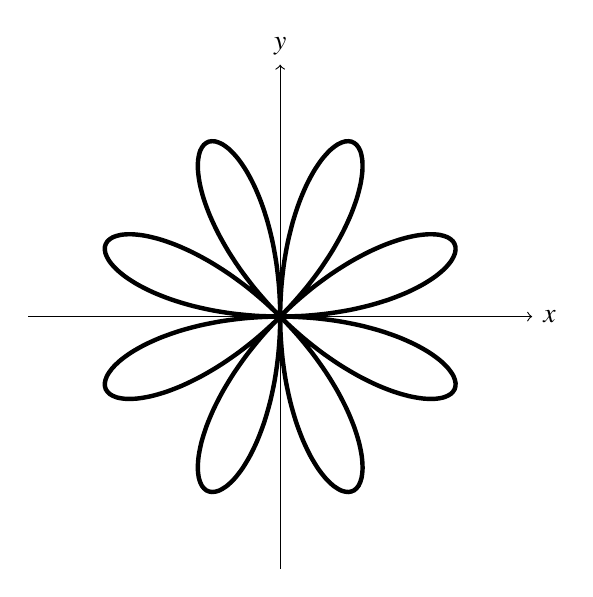
\begin{tikzpicture}[scale=0.8]
    % Draw axes
    \draw[->] (-4,0) -- (4,0) node[right] {$x$};
    \draw[->] (0,-4) -- (0,4) node[above] {$y$};
    
    % Draw the polar curve r = 3*sin(2*theta)
    \draw[ultra thick, domain=0:360, samples=200, smooth]
        plot ({3*sin(4*\x)*cos(\x)}, {3*sin(4*\x)*sin(\x)});
\end{tikzpicture}
\vfill
\newpage
Extra Credit (5 points) Let $f(x) = \displaystyle{\sum_{n=0}^\infty { \frac{1}{2} \choose n} \frac{x^n}{3^n}}.$
	\begin{enumerate}
	\item Determine the first 4 terms in the series. Simplify the coefficients.
	\vfill
	\item The series converges when $x=2.$ Determine the sum.
	\vfill
	\end{enumerate}
\end{enumerate}
\end{document}
